% !TEX encoding = UTF-8
% !TEX TS-program = pdflatex
% !TEX root = ../Articolo.tex
% !TEX spellcheck = it-IT

%************************************************
\section{Behavior Investigation}
\label{section:behaviorinvestigation}
%************************************************

This is the fourth draft of what should be the main topic of my PhD Thesis. 
The \textbf{ToC} is developed accordingly and attached.

\subsection{Investigation topcis}
\label{subsection:investigationtopics}

The scientific core of my PhD Thesis will investigate the following themes:
\begin{enumerate}
\item{the influence of variations (distributions) of input parameters,}
%\item{the behavior of the different properties in real life (e.g. segregation before doing the shear cell experiment),}
\item{the influence of and poly-dispersity, i.e. the possbility to extrapolate
(e.g. given 3 different fraction distributions, with known behaviors, extrapolate 
the behavior of a fourth fraction distribution).}
\end{enumerate}

\begin{figure}[!h]
\centering
\subfloat[Regression coefficient of internal friction - polidispersity ANN]
{\label{fig:041regressionavg1}
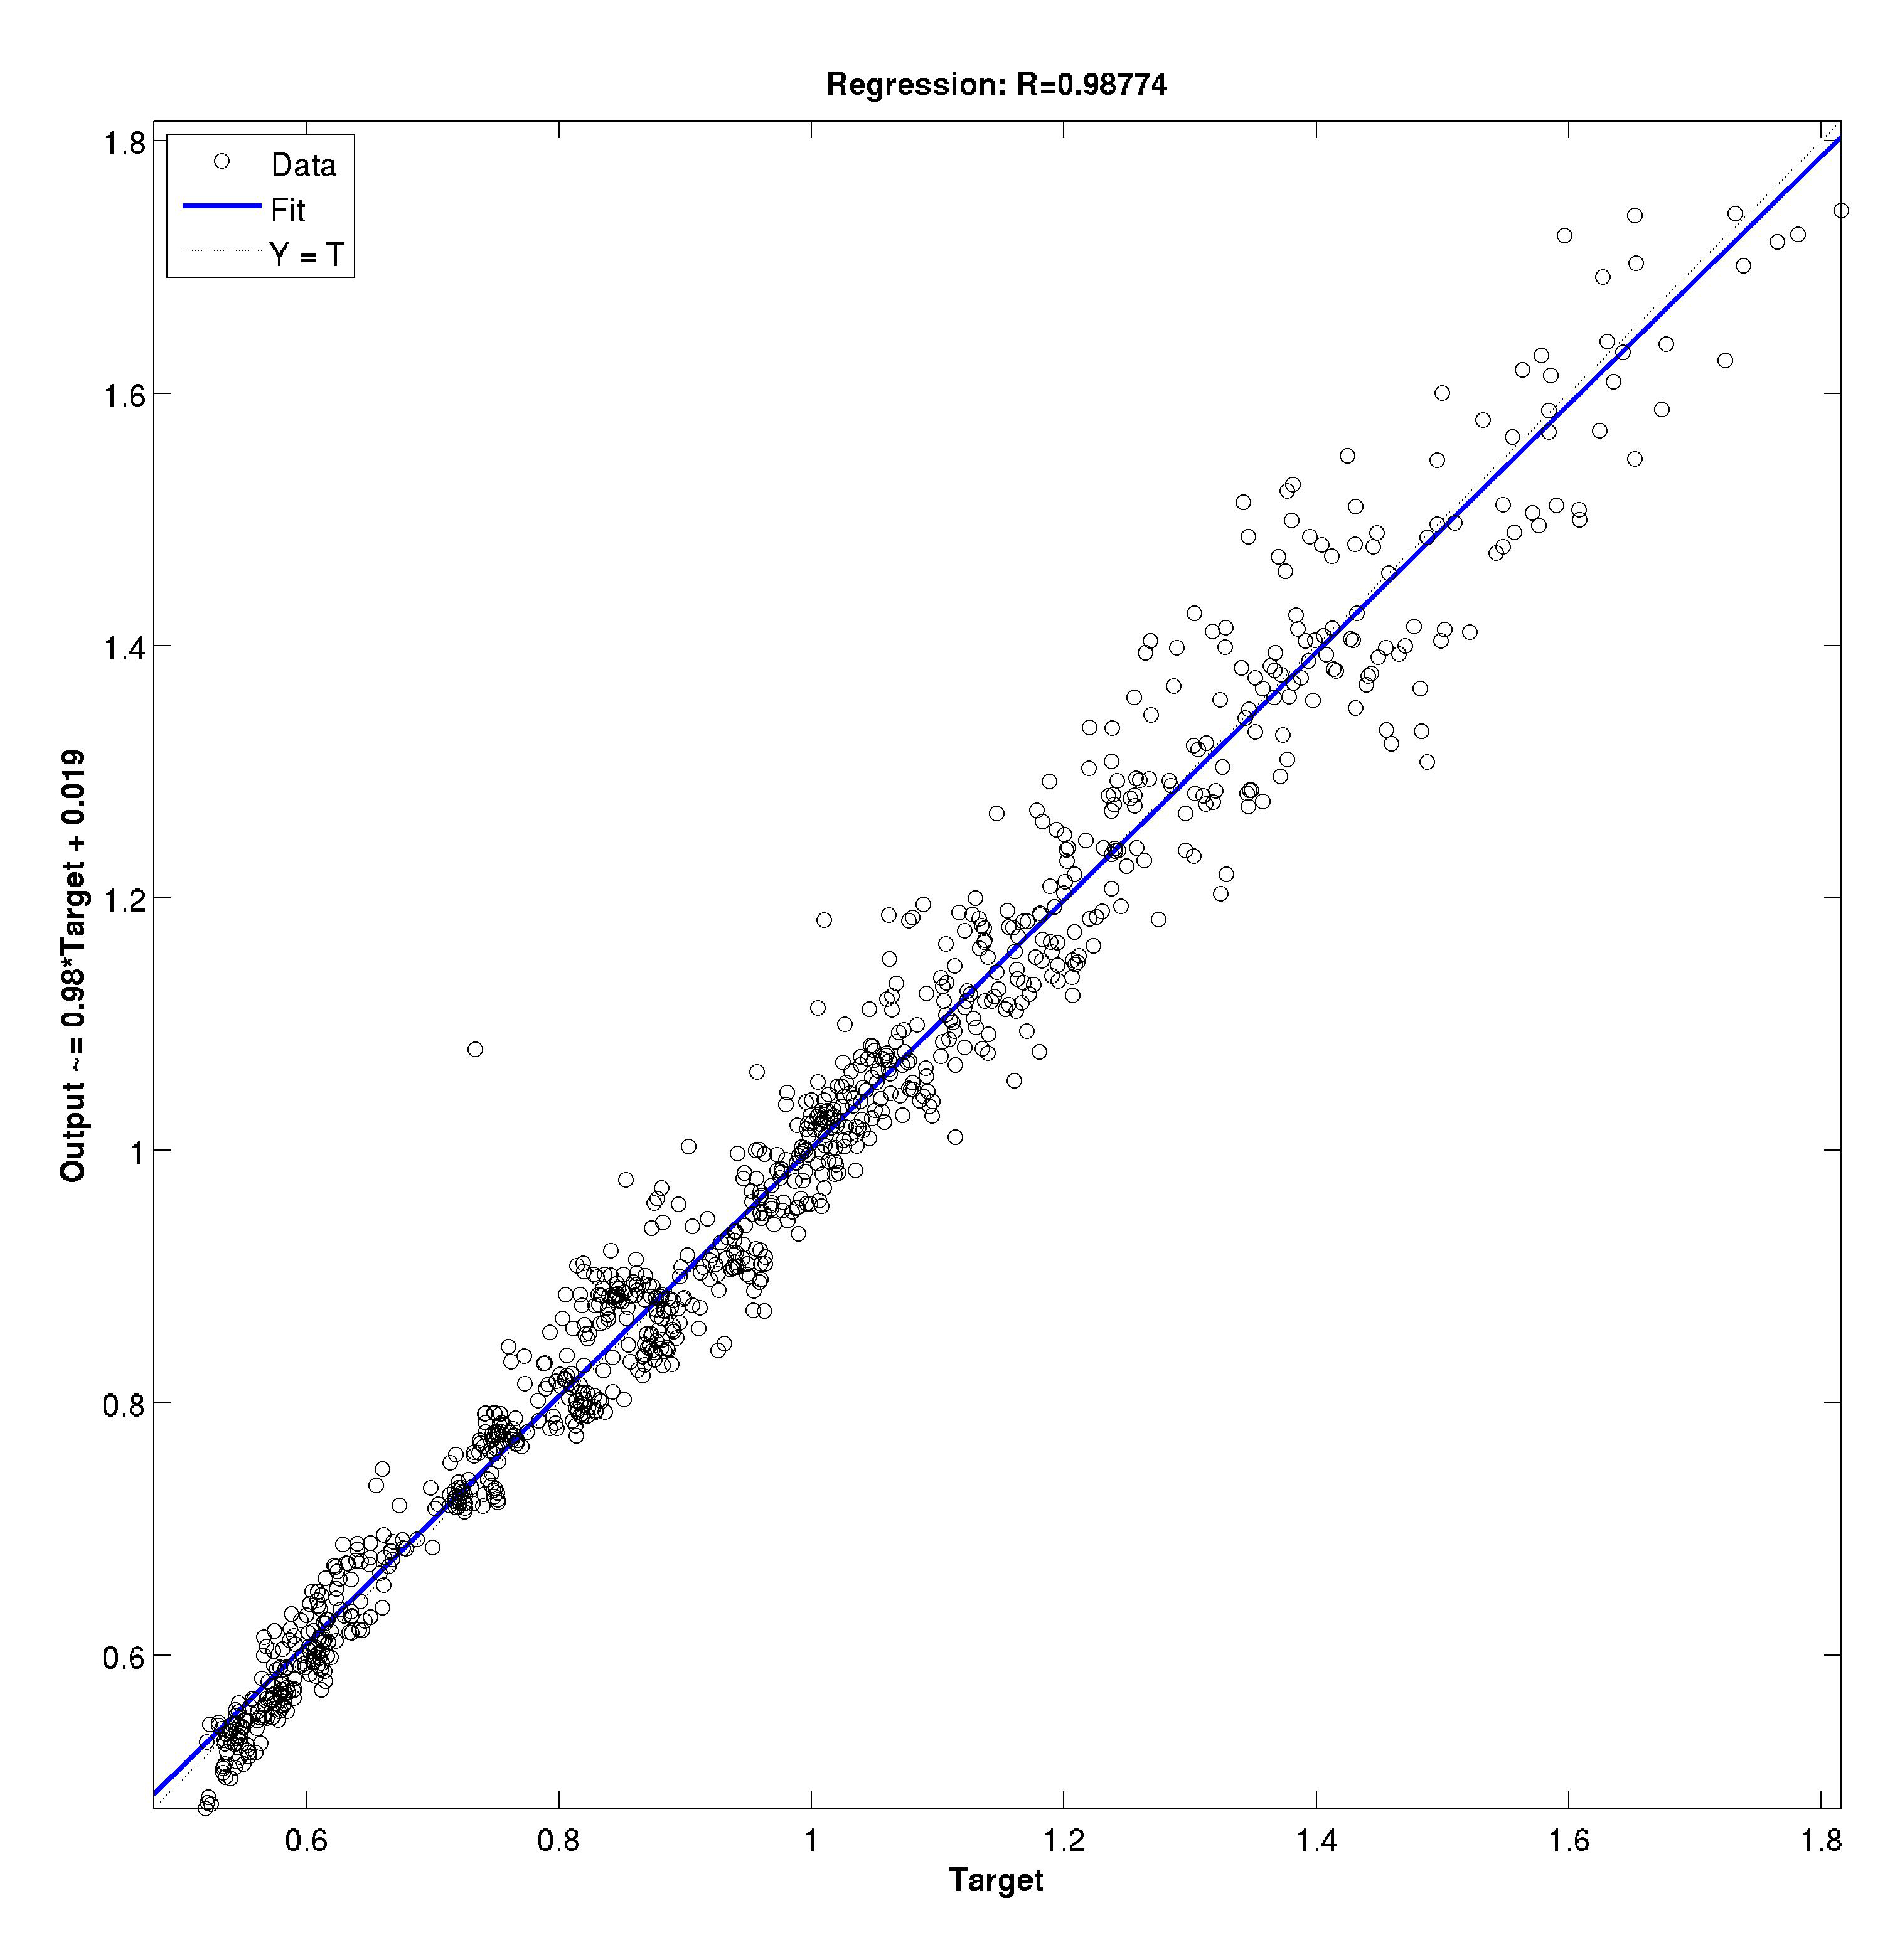
\includegraphics[width=.35\columnwidth]{041regressionavg1}} \\
\subfloat[Radius distribution with 1st simulation set]
{\label{fig:046simulationRadiusDistribution5}
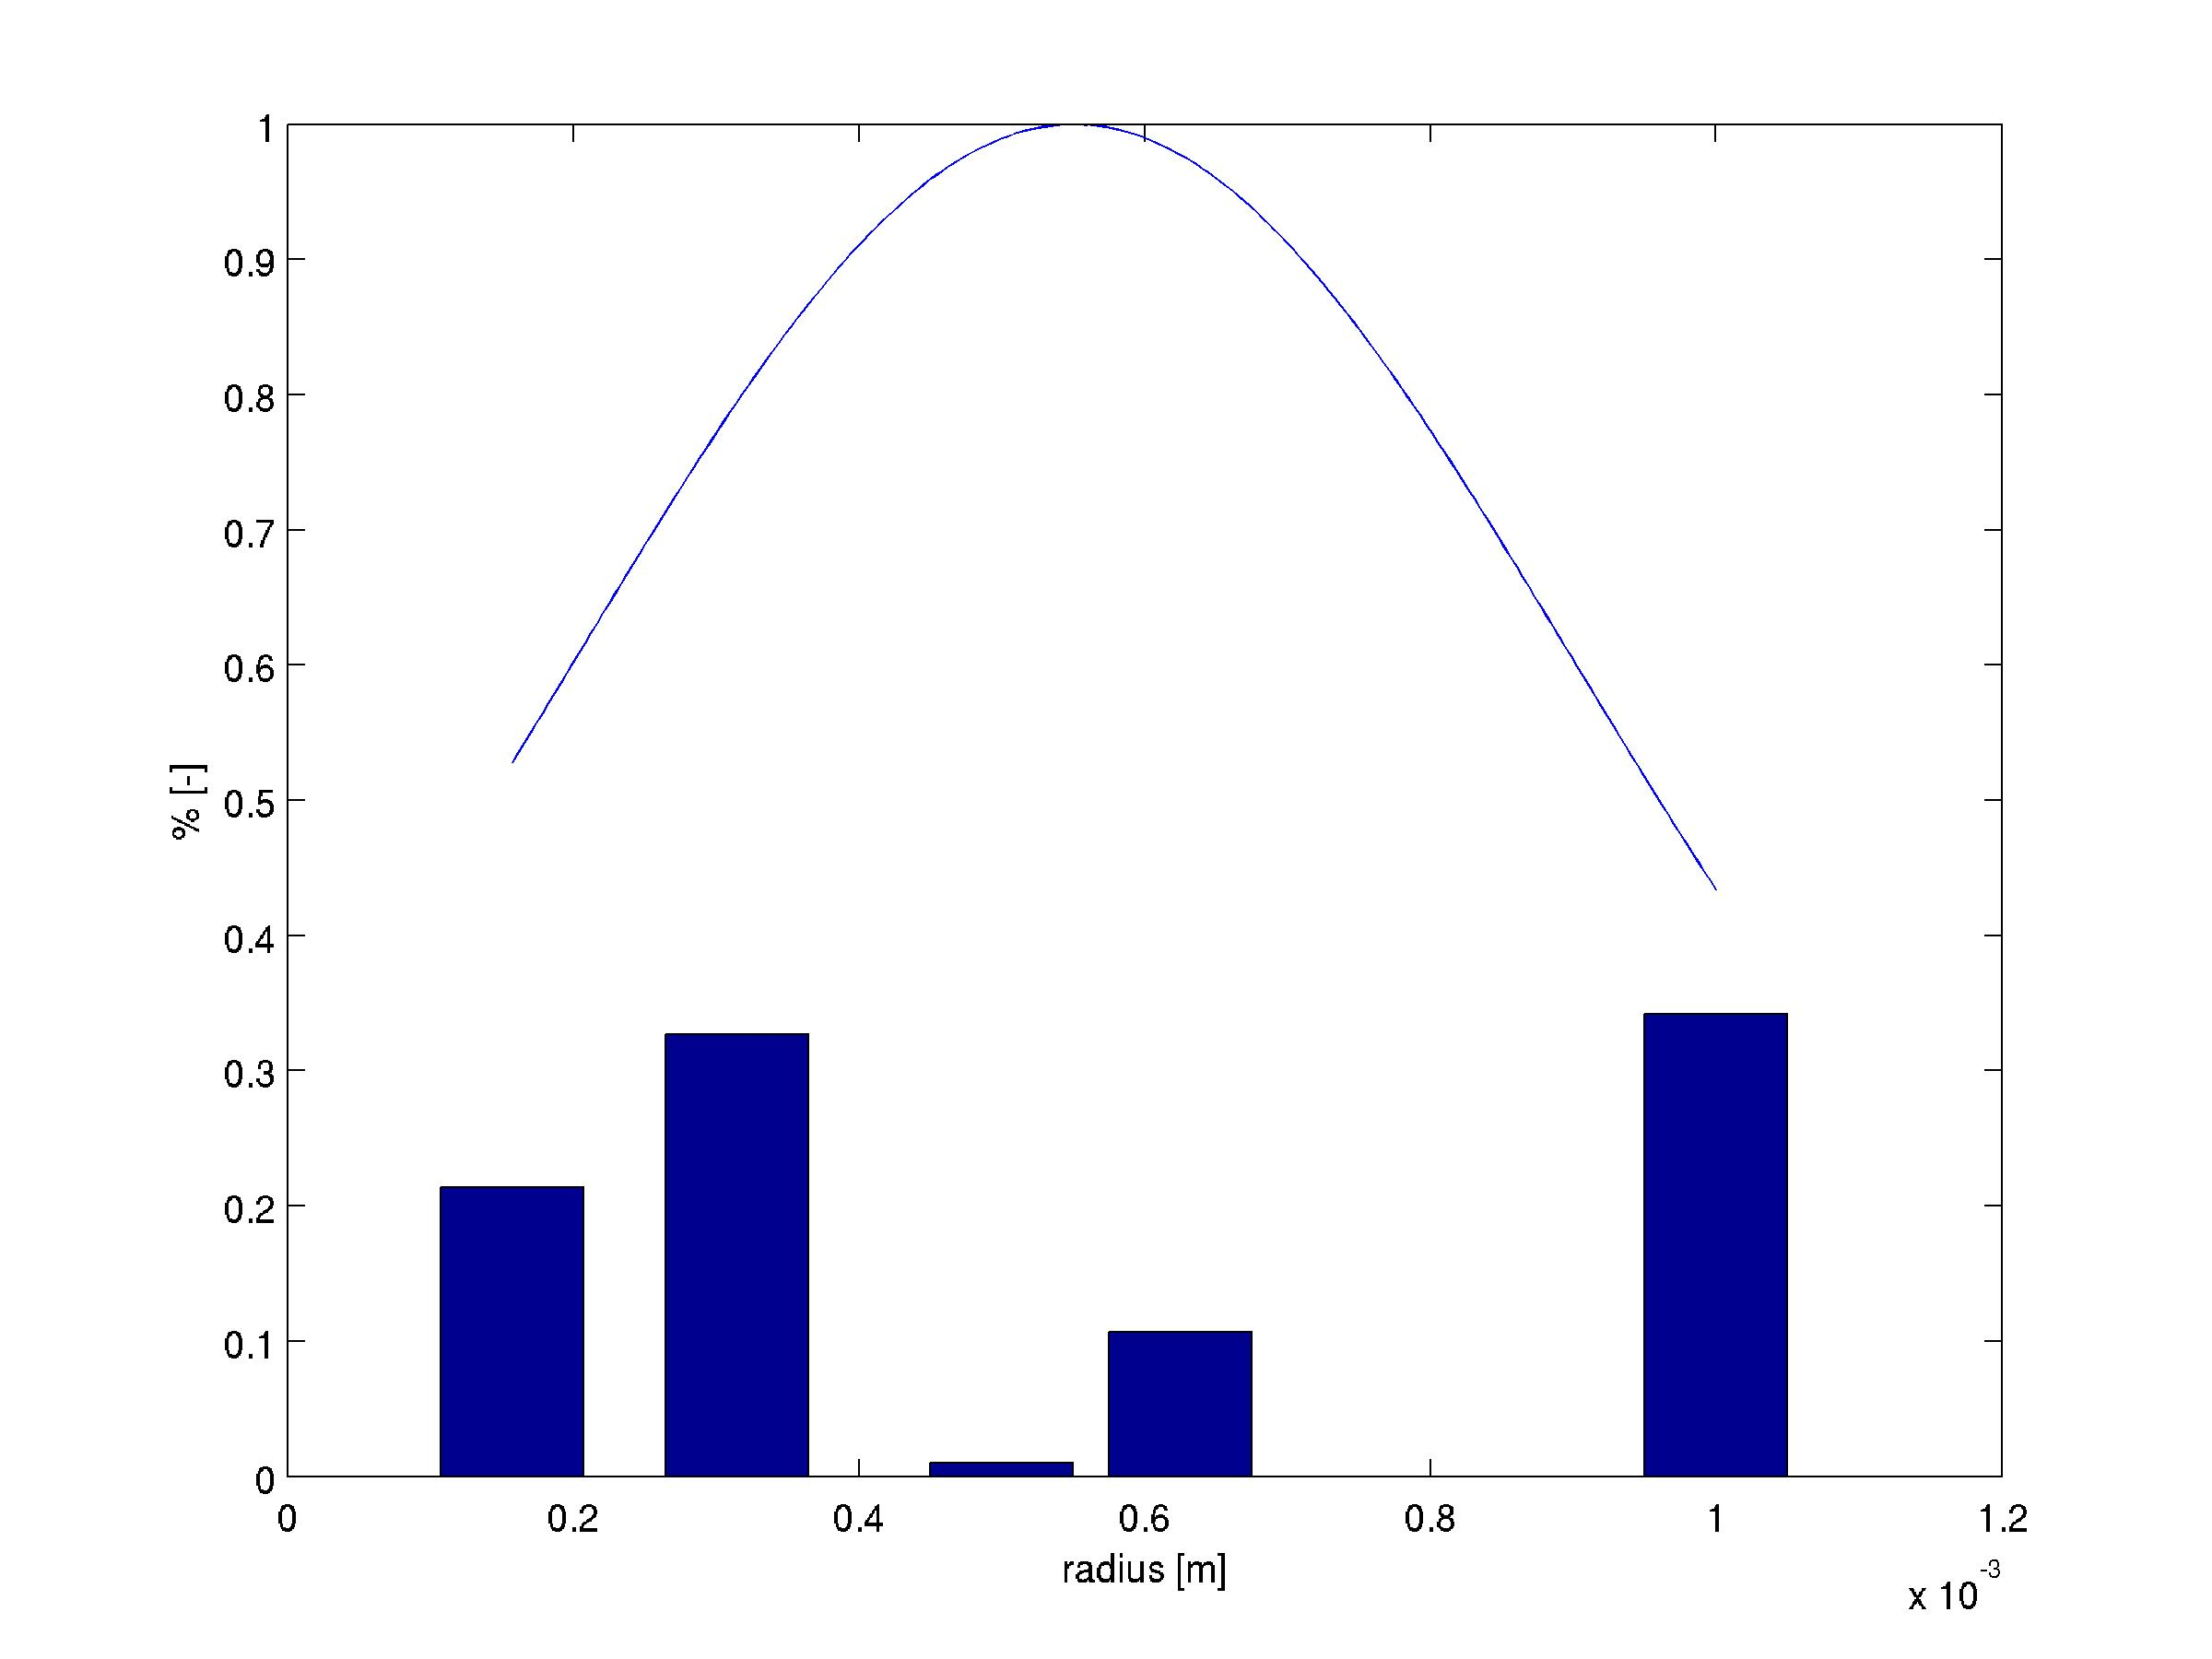
\includegraphics[width=.35\columnwidth]{046simulationRadiusDistribution5}} \quad
\subfloat[Radius distribution with 2nd simulation set]
{\label{fig:047simulationRadiusDistribution6}
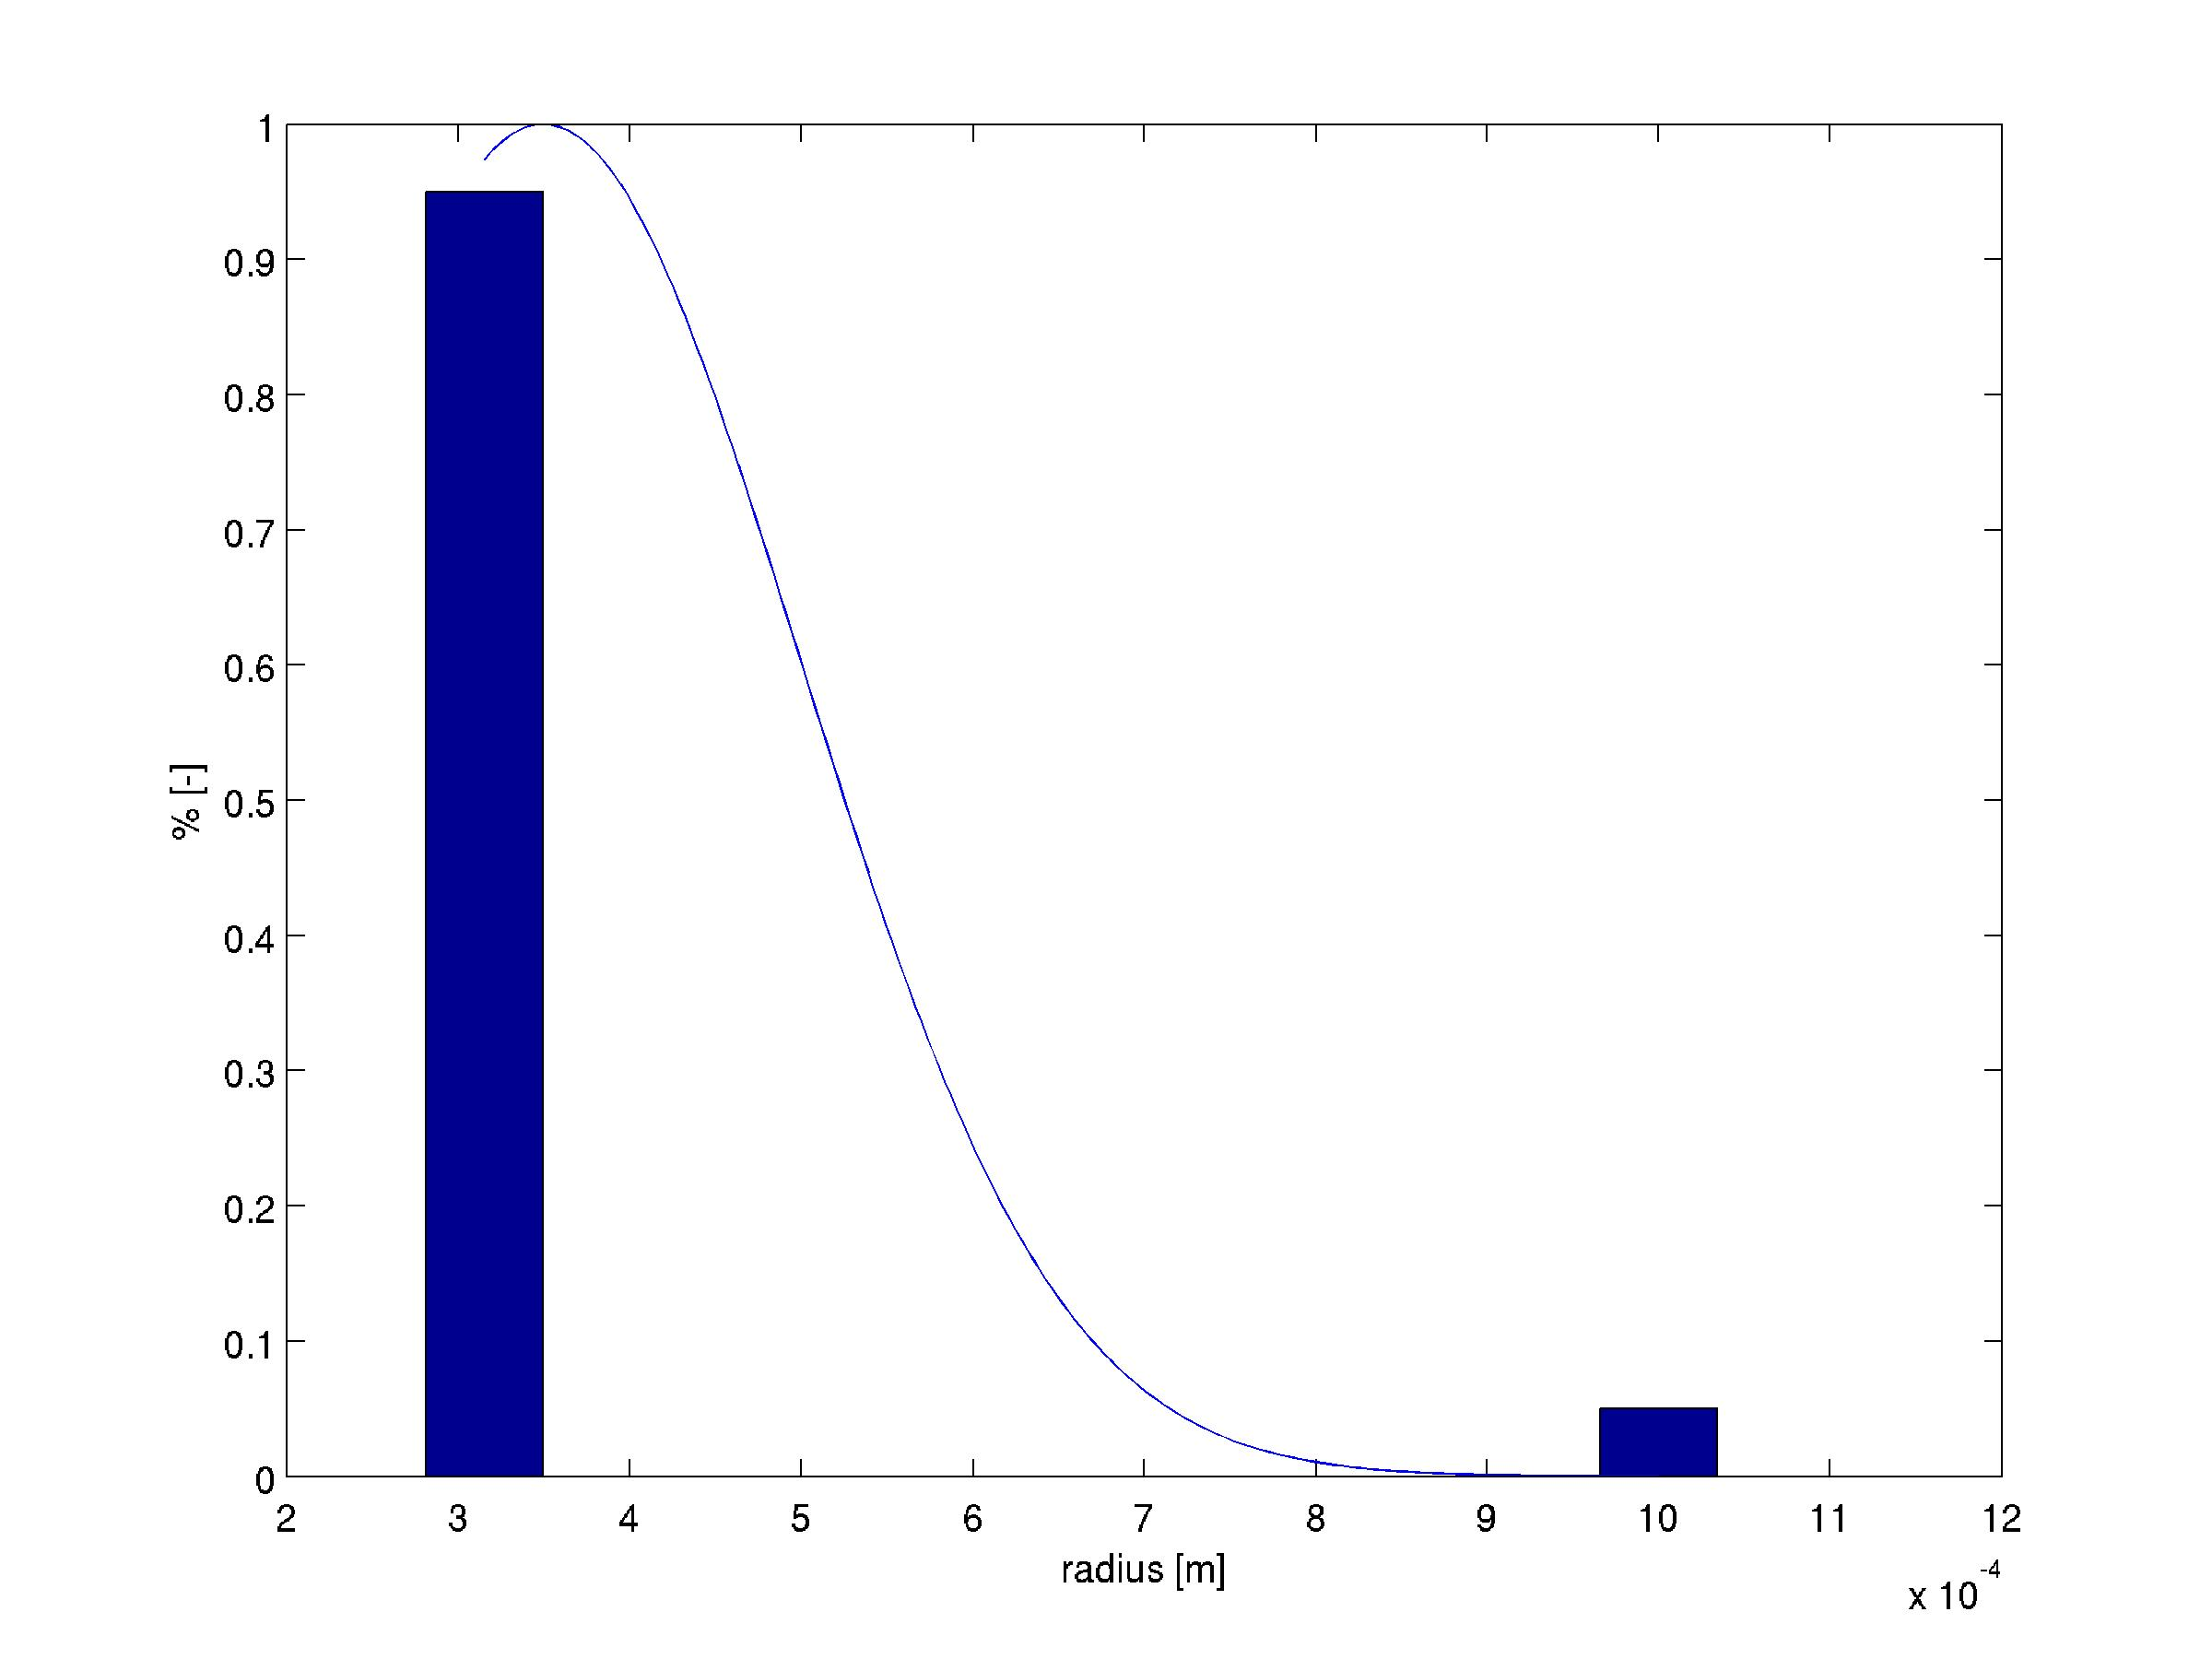
\includegraphics[width=.35\columnwidth]{047simulationRadiusDistribution6}} \\
\subfloat[Radius distribution with 3rd simulation set]
{\label{fig:048simulationRadiusDistribution7}
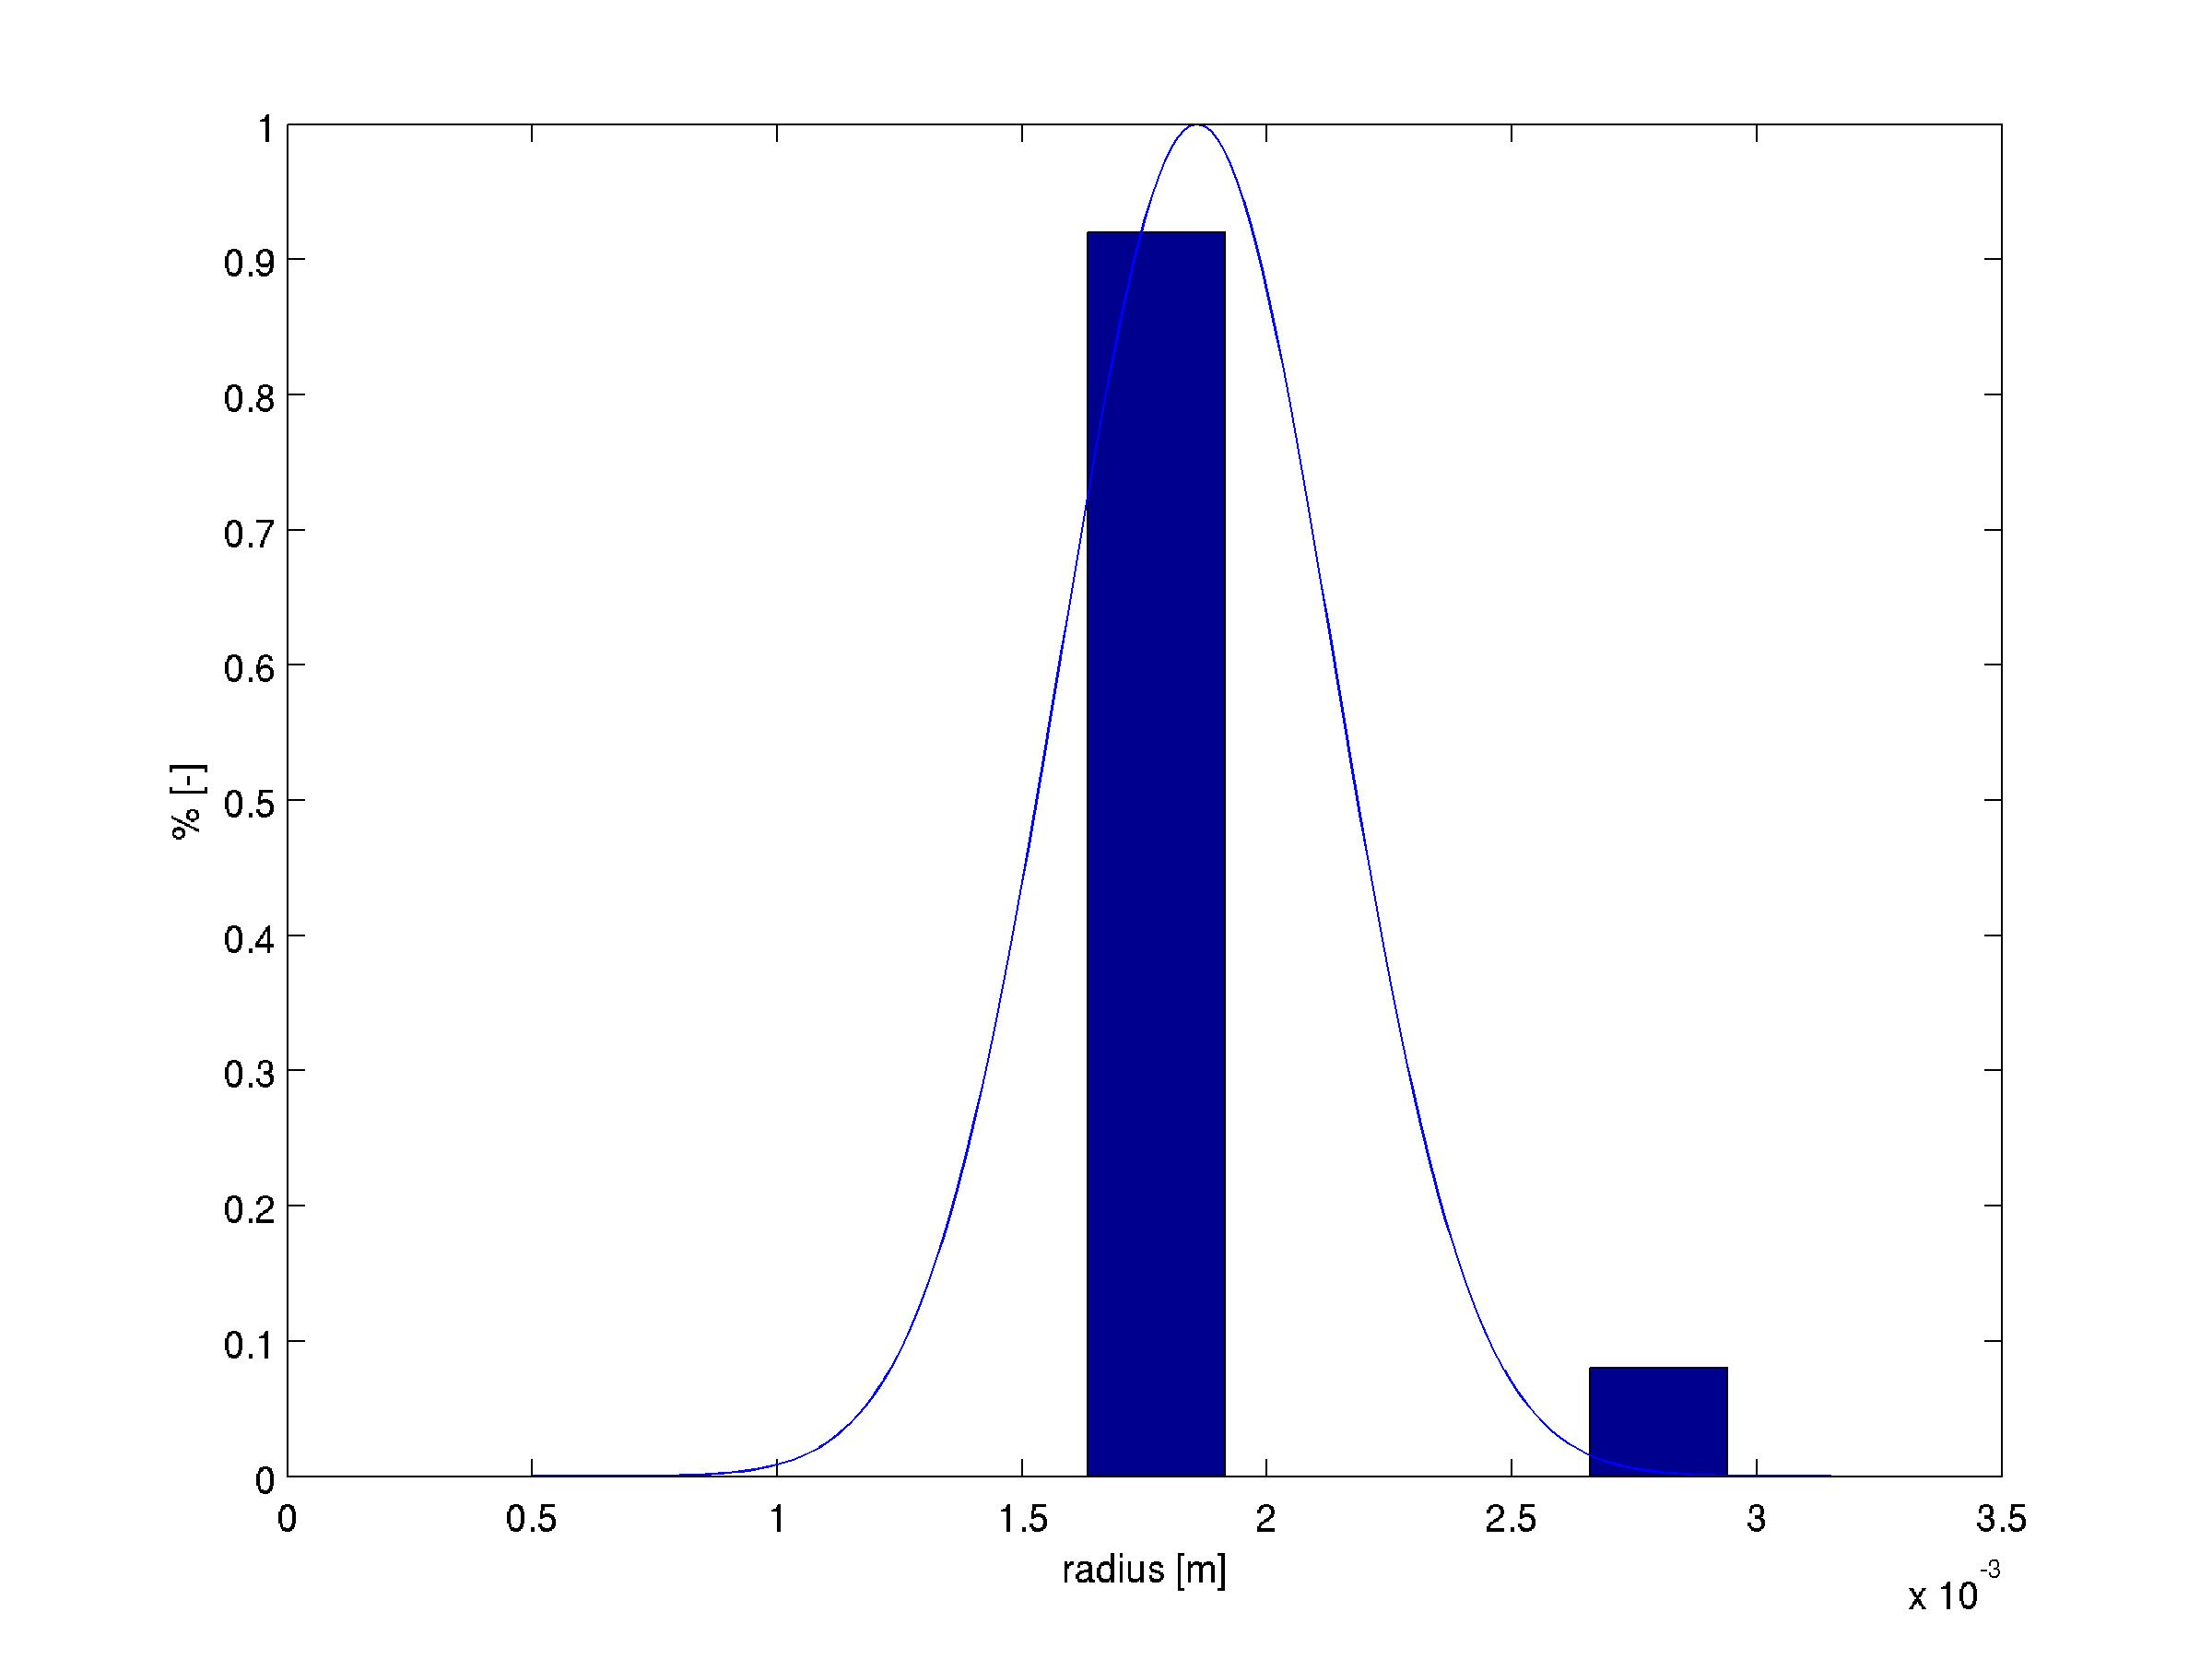
\includegraphics[width=.35\columnwidth]{048simulationRadiusDistribution7}} \quad
\subfloat[Radius distribution with 4th simulation set]
{\label{fig:049simulationRadiusDistribution8}
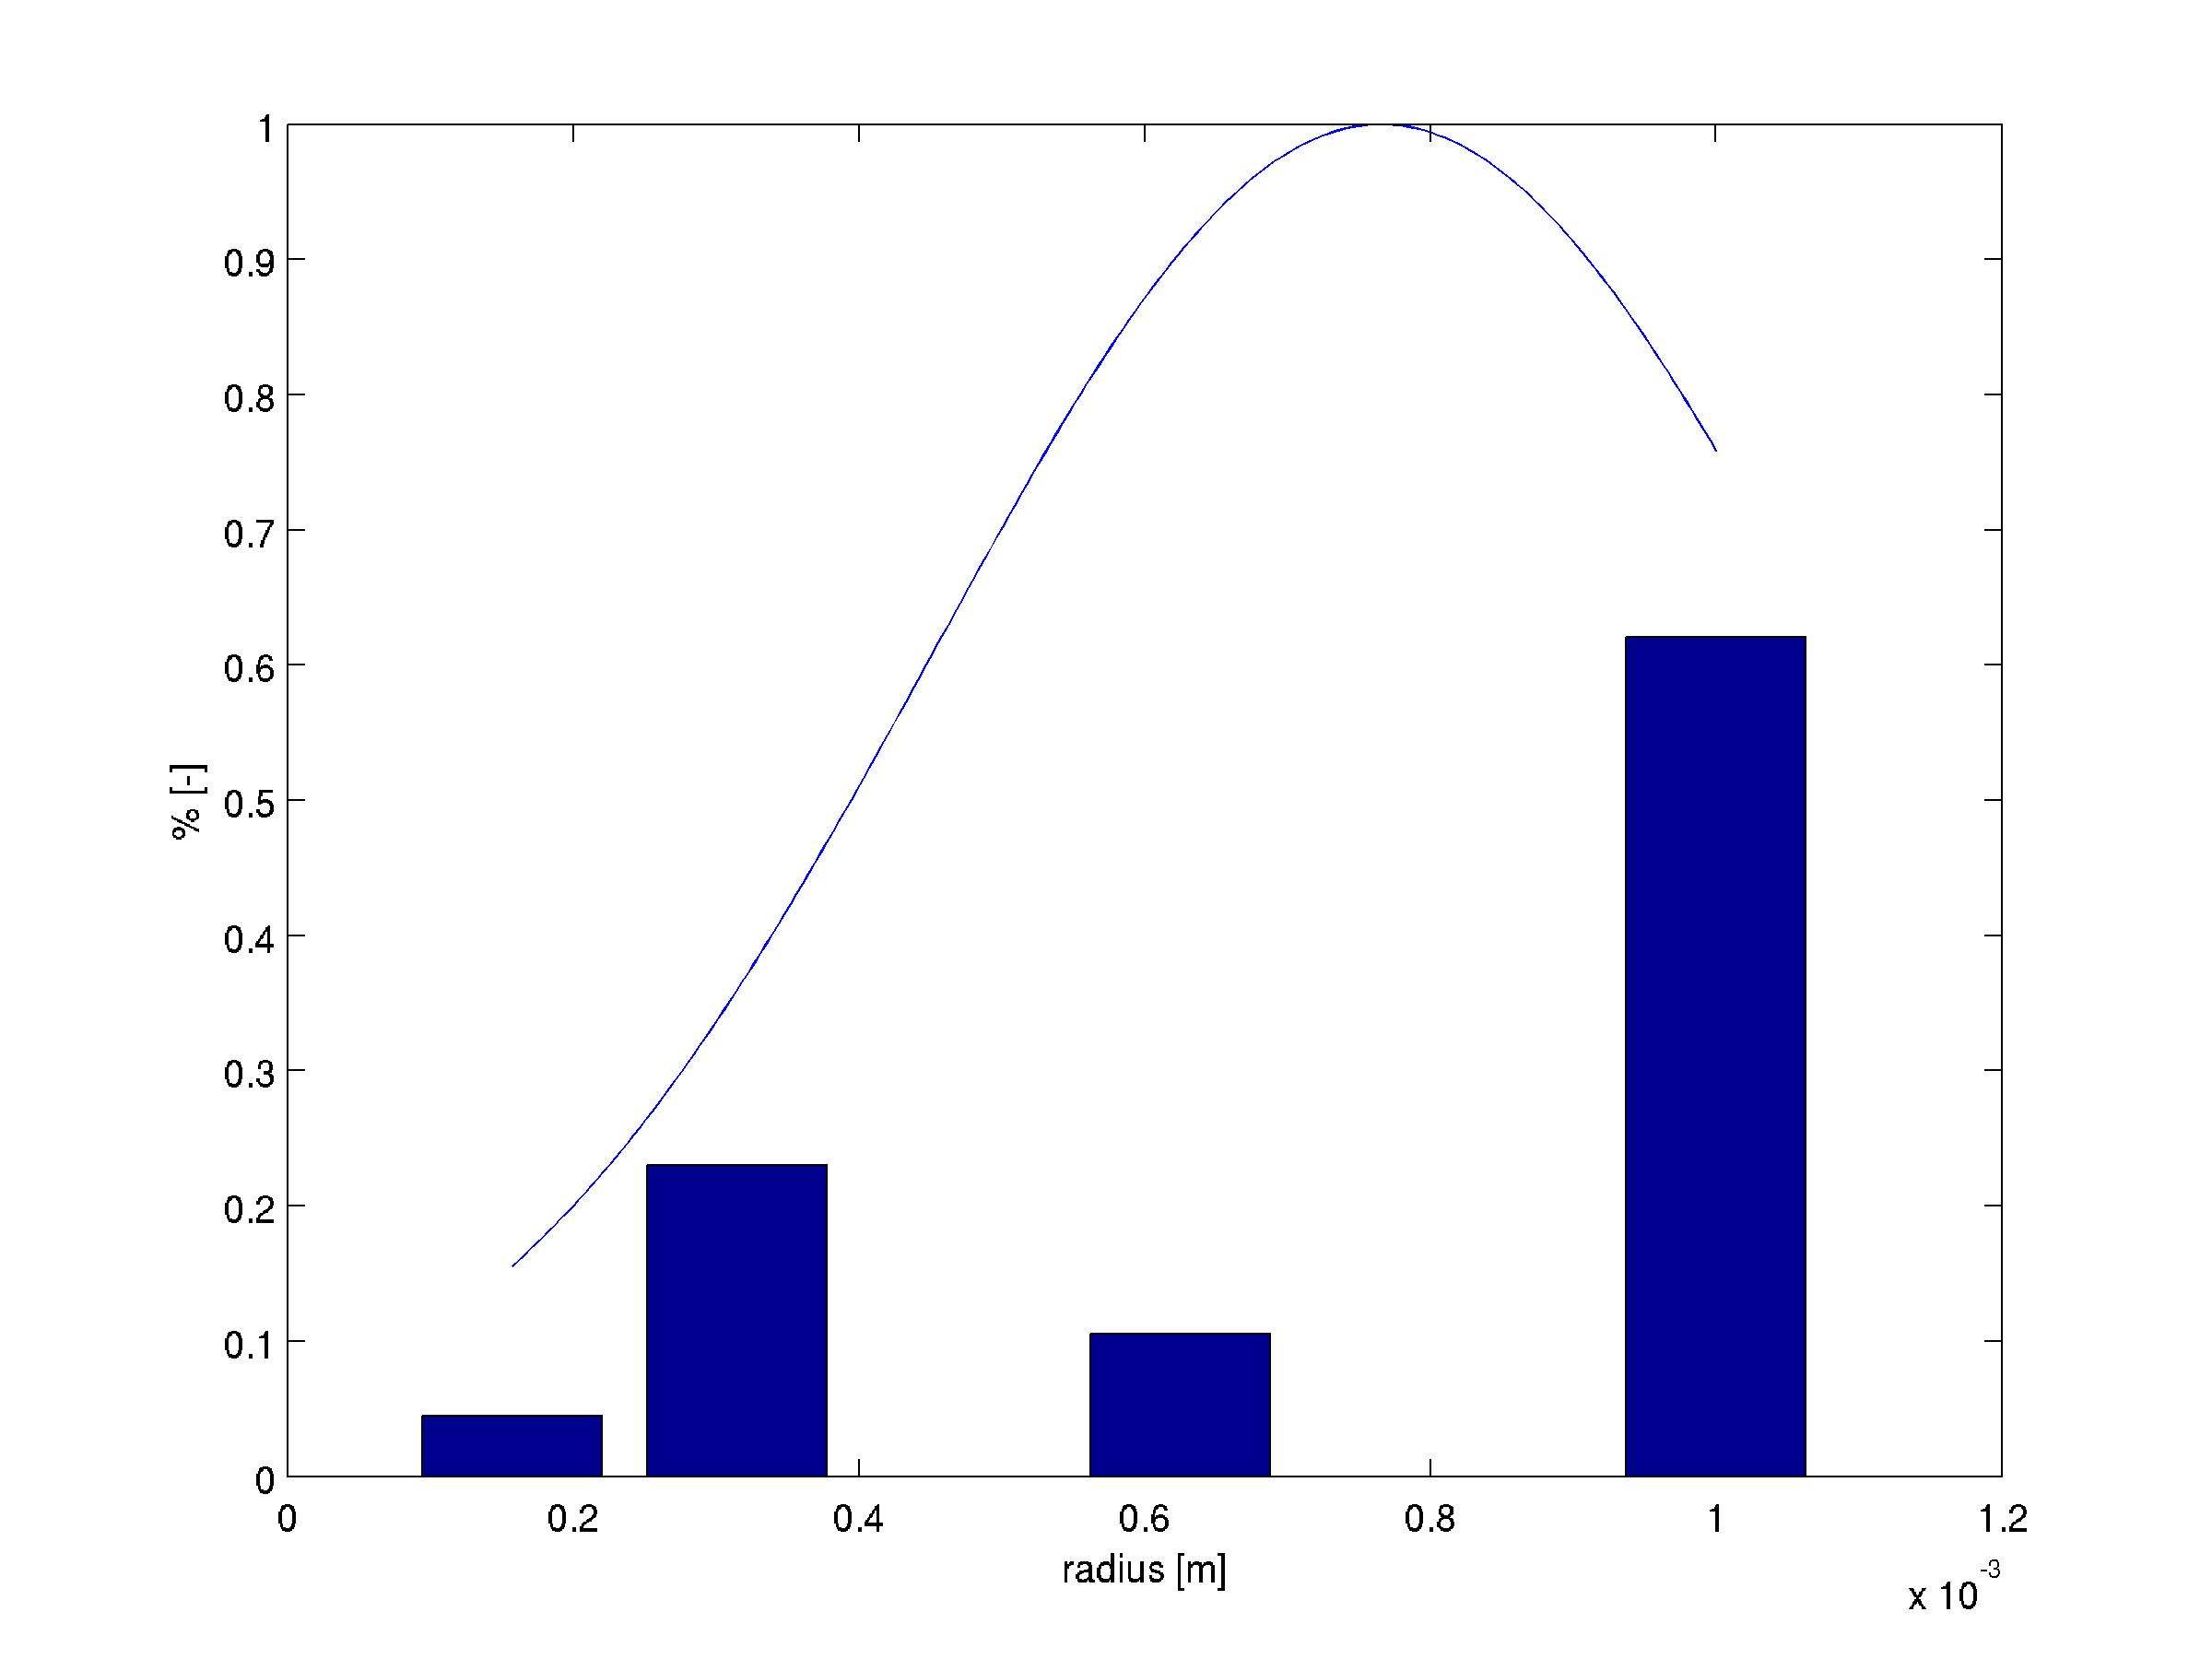
\includegraphics[width=.35\columnwidth]{049simulationRadiusDistribution8}} \\
\subfloat[Radius distribution with minimum standard deviation]
{\label{fig:042minStdDevRad}
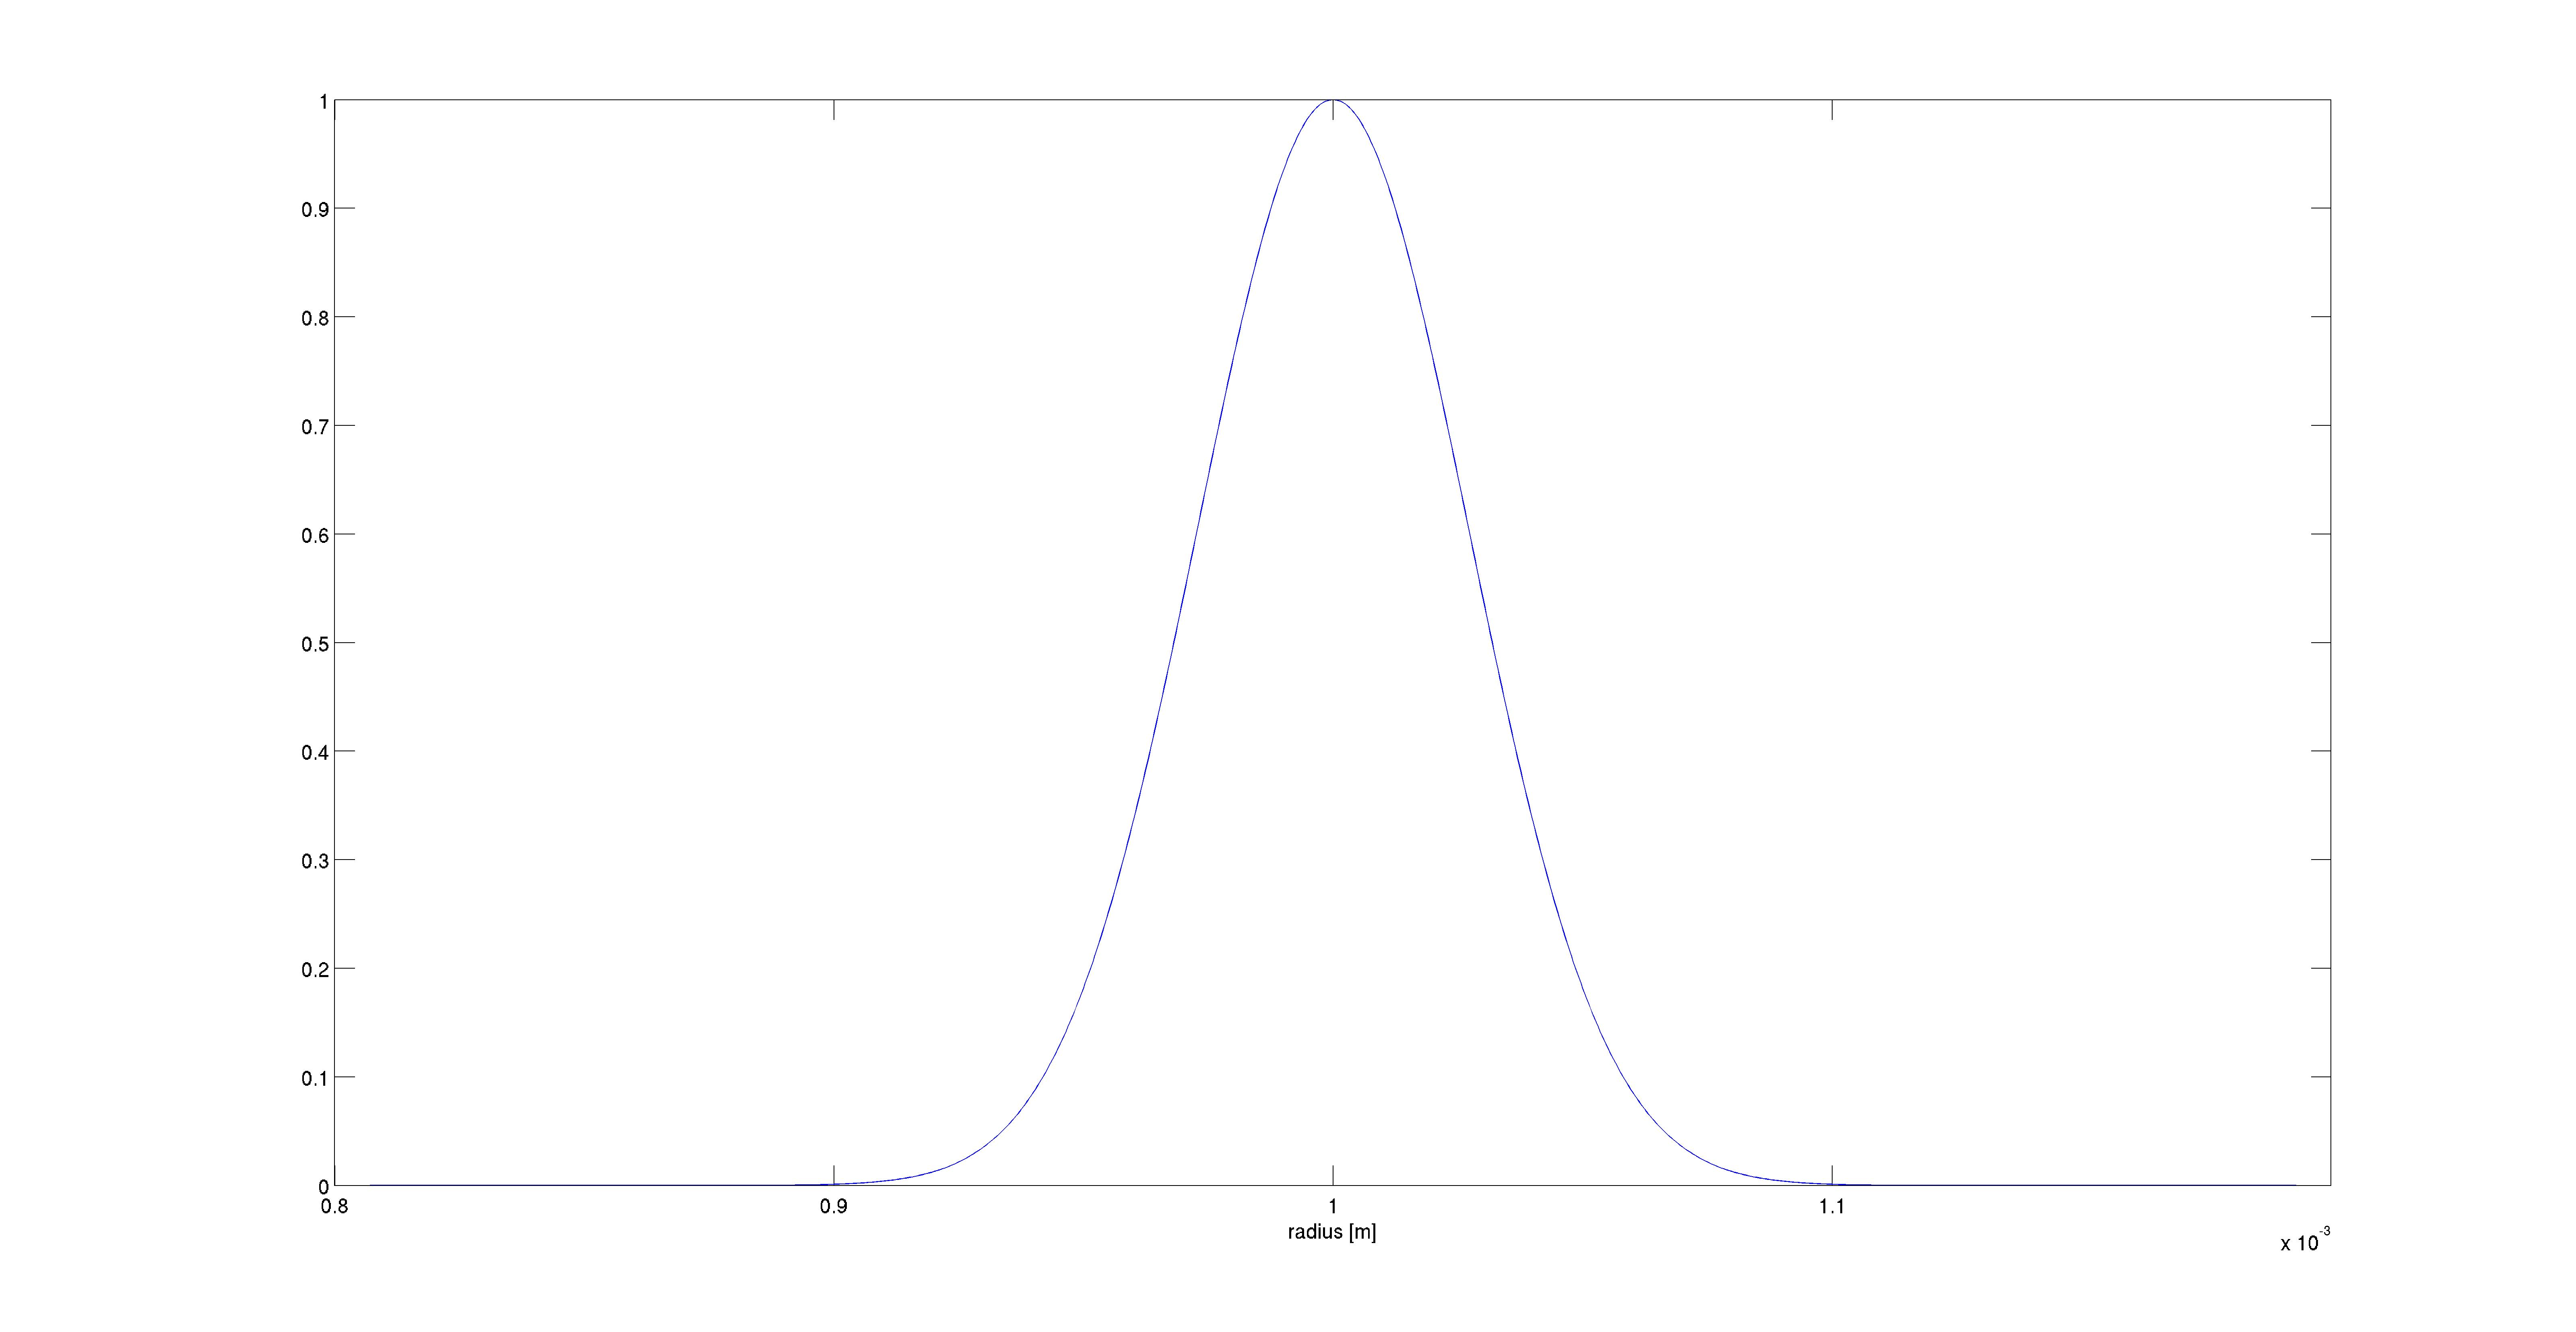
\includegraphics[width=.35\columnwidth]{042minStdDevRad}} \quad
\subfloat[Radius distribution with maximum standard deviation]
{\label{fig:043maxStdDevRad}
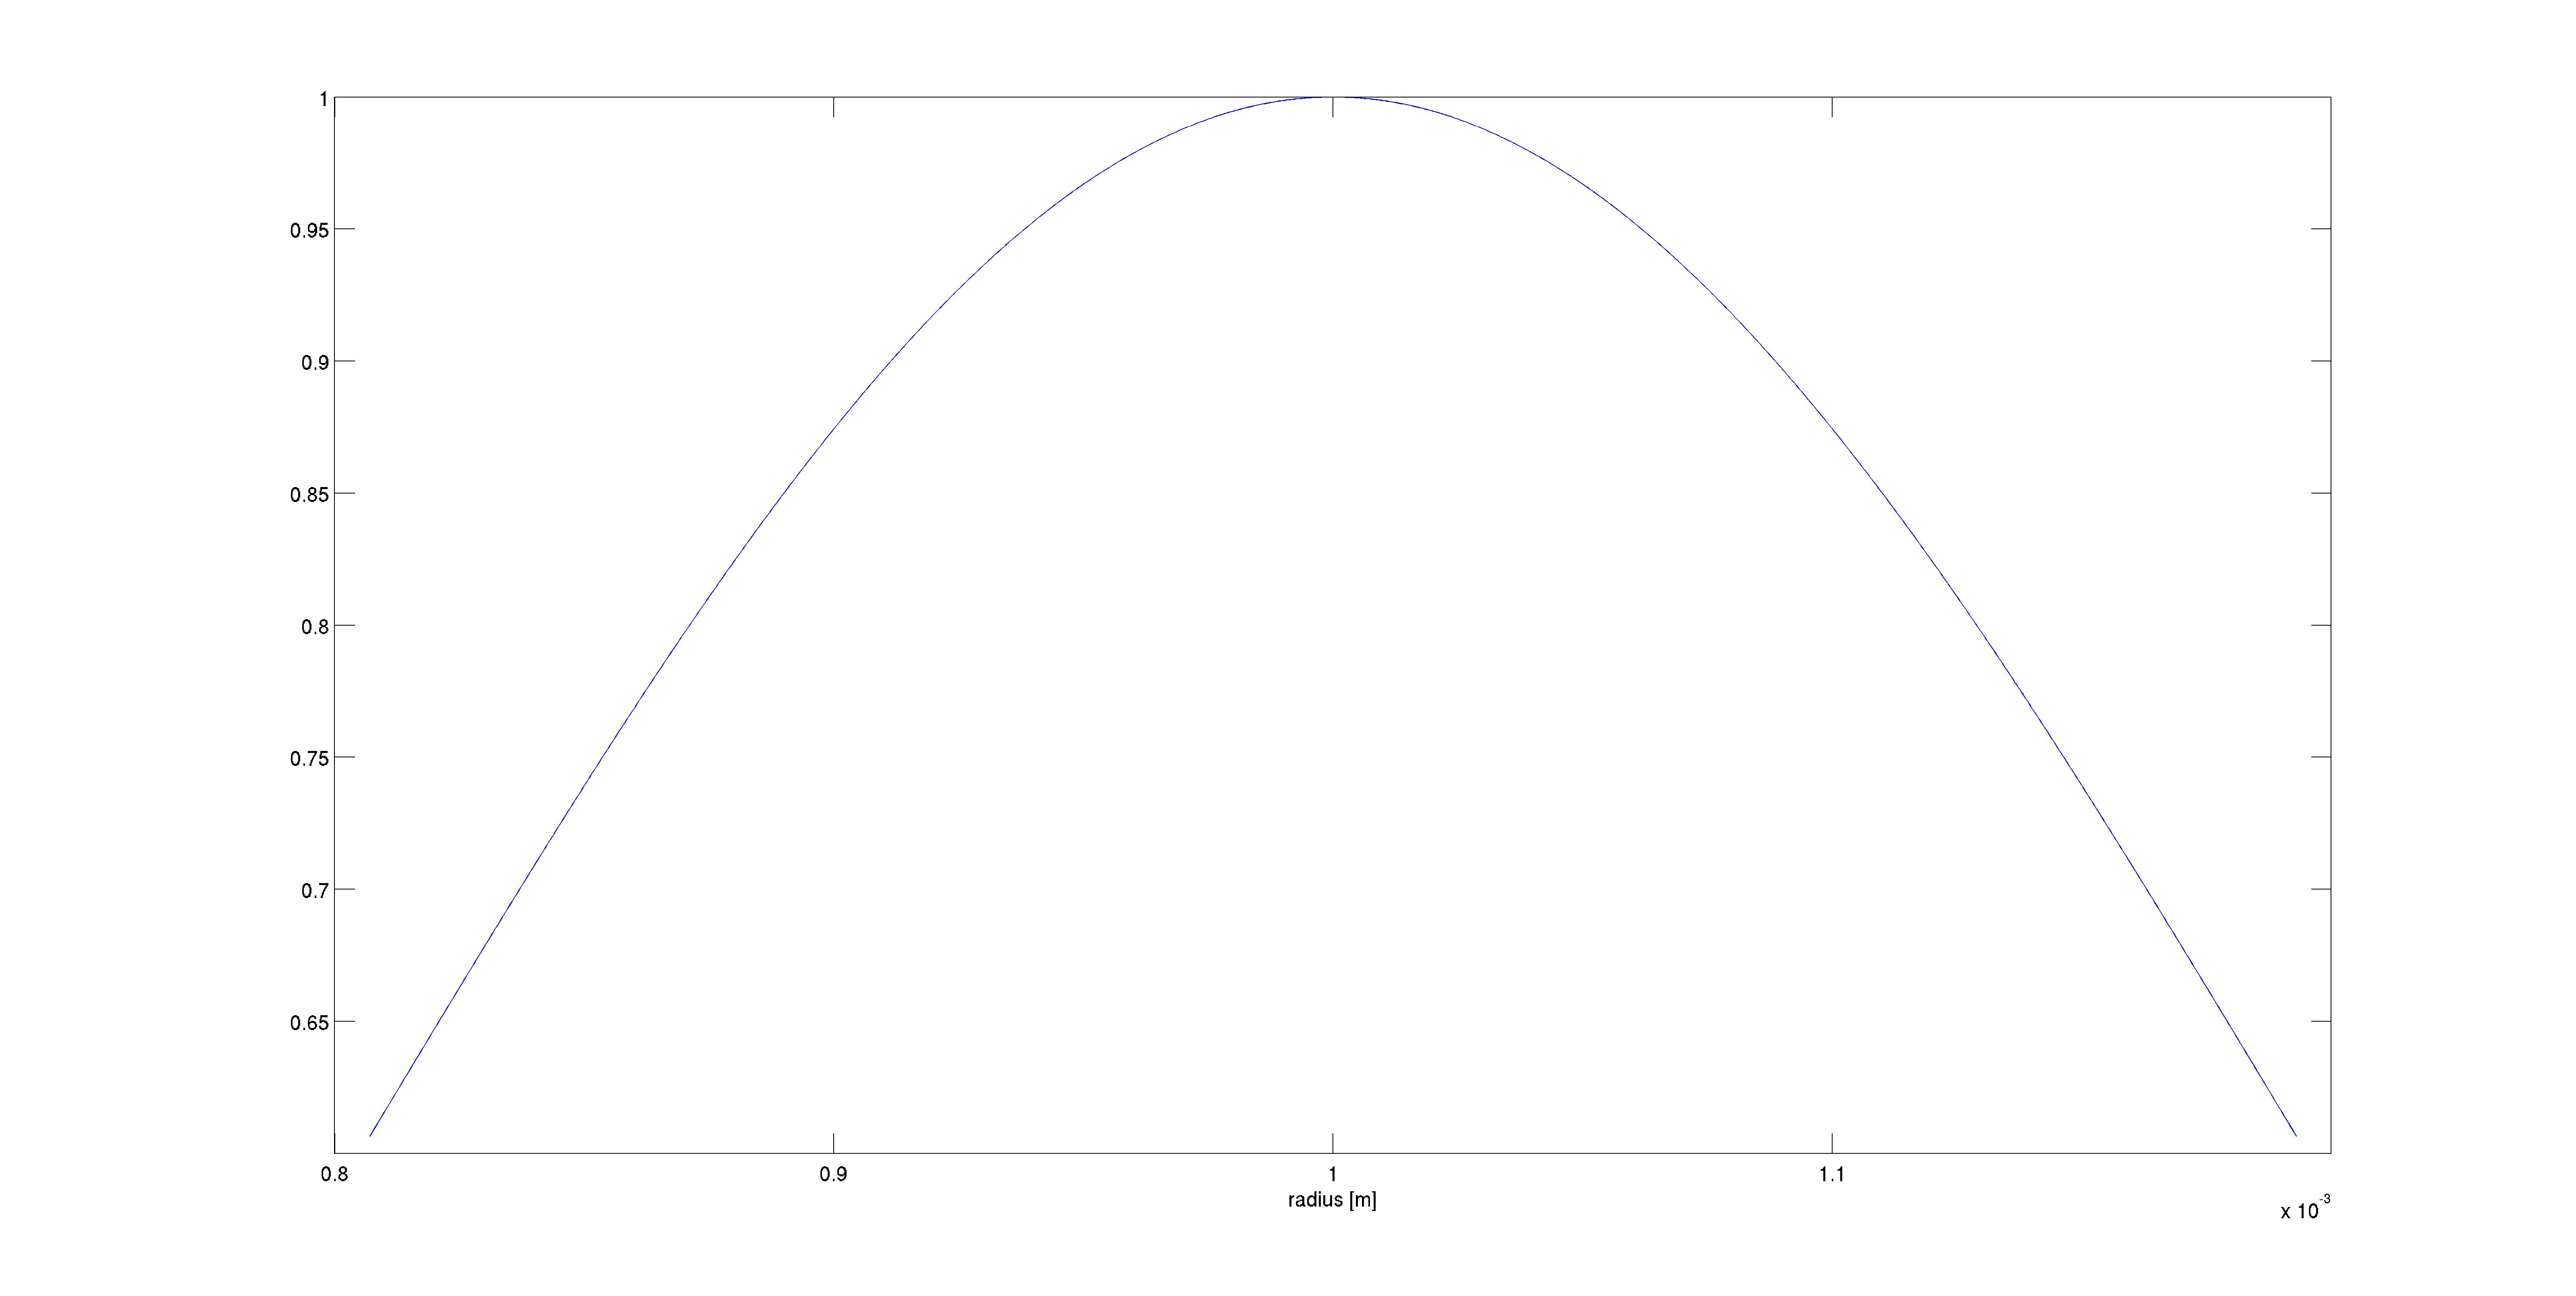
\includegraphics[width=.35\columnwidth]{043maxStdDevRad}} 
\caption[ANN and std dev radius]{ANN and std dev radius}
\label{fig:annandstddevradius}
\end{figure}

\subsection{Artificial neural network}
\label{subsection:artificialneuralnetwork}

The first core item has been completed for sinter fine with dedicated Artificial
neural networks ($ANNs$), that has been described in a journal paper draft, see
\ref{sec:elsevierpaper}.\\

I have started the second core item, I have used the polidispersity information
available (mean and standard deviation of the radius) for the simulations
already performed to train another series of $ANNs$, see Fig.
\ref{fig:annandstddevradius}.\\
Later I gave to the $ANNs$ input combinations with combinations that had a mean radius of 1 mm
and 50 different std dev, varying from 2.71e-05 m to 1.93e-04 m.
The minimum and maximum values are plotted in Fig. \ref{fig:042minStdDevRad} and
\ref{fig:043maxStdDevRad} respectively.\\
The variation of the bulk values (adimensional) against the std dev of the
radius calculated by the three $ANNs$ can be seen in Fig. \ref{fig:044bulkMean}:
the bulk density and the coefficient of internal friction after
compaction respond according to theory (more dispersion --> more small particles
--> higher compaction --> higher density and friction).
The coefficient of internal friction before compaction does not.
I am investigated this issue by creating a new, dedicated, $DEM$ simulations
set.


\begin{figure}[!h]
\centering
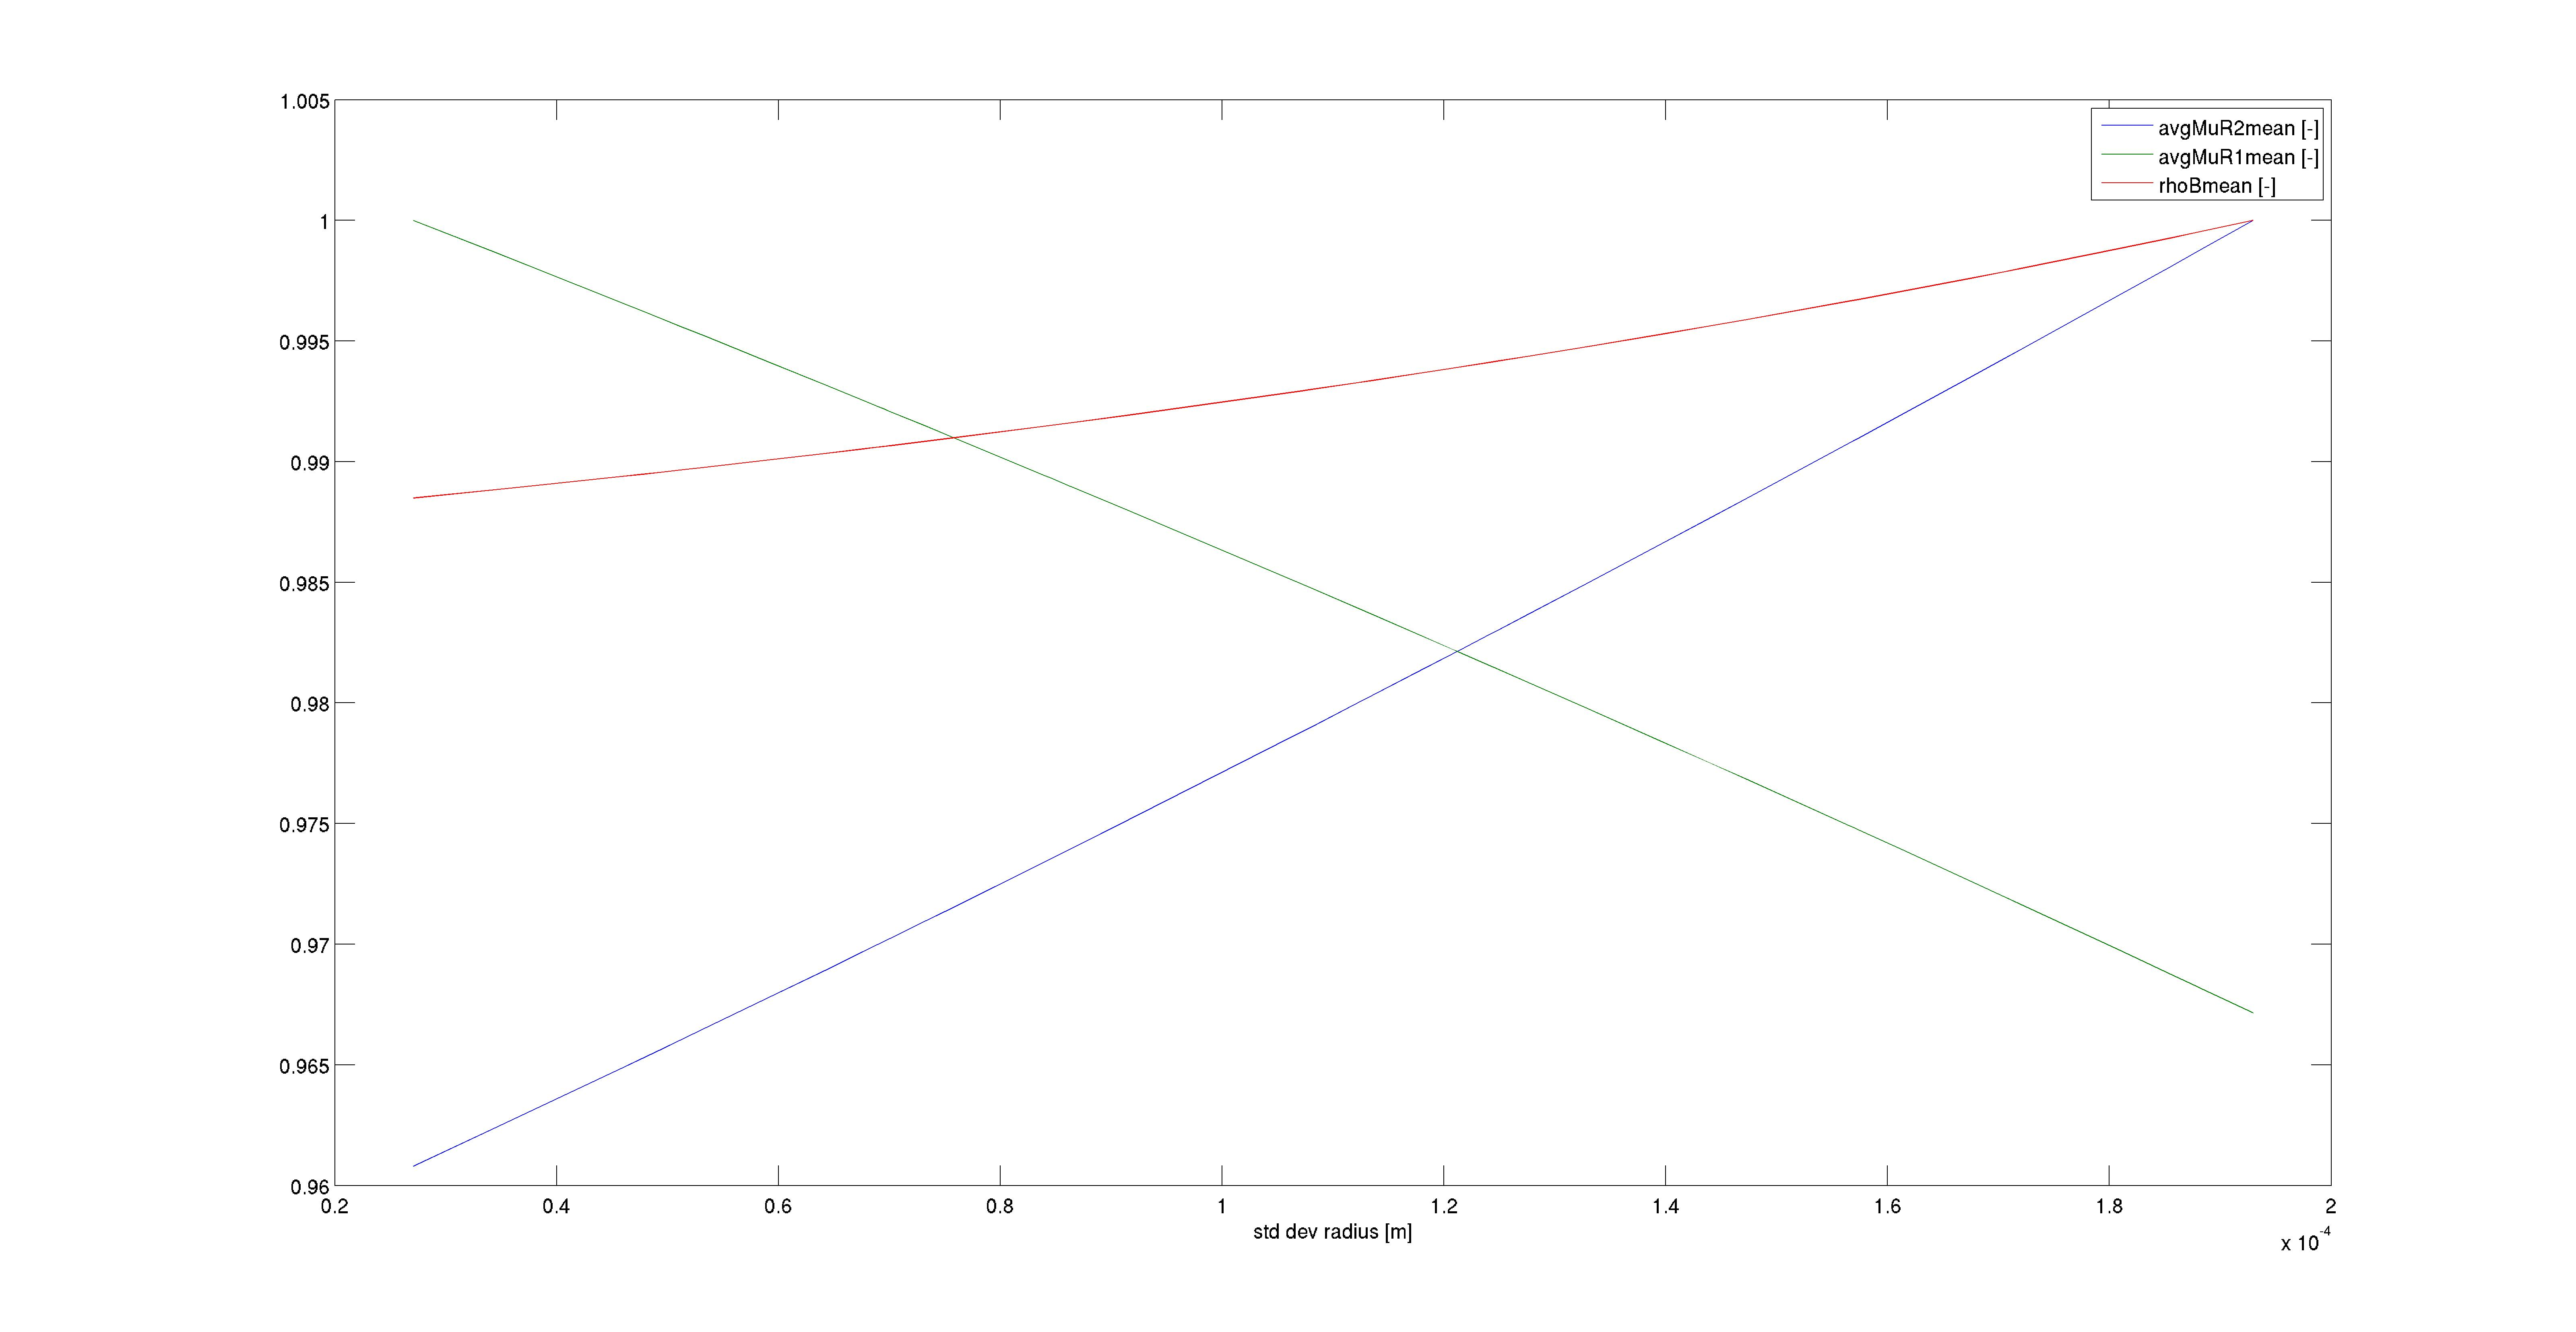
\includegraphics[width=.96\columnwidth]{044bulkMean}
\caption{Variation of bulk values }
\label{fig:044bulkMean}
\end{figure}

\newpage
